%\usepackage{subcaption}
%\usepackage{sectsty}
%\allsectionsfont{\normalfont\scshape} 
%\input{tcilatex}
%\input{tcilatex}


\documentclass[superscriptaddress, notitlepage]{revtex4-1}
%%%%%%%%%%%%%%%%%%%%%%%%%%%%%%%%%%%%%%%%%%%%%%%%%%%%%%%%%%%%%%%%%%%%%%%%%%%%%%%%%%%%%%%%%%%%%%%%%%%%%%%%%%%%%%%%%%%%%%%%%%%%%%%%%%%%%%%%%%%%%%%%%%%%%%%%%%%%%%%%%%%%%%%%%%%%%%%%%%%%%%%%%%%%%%%%%%%%%%%%%%%%%%%%%%%%%%%%%%%%%%%%%%%%%%%%%%%%%%%%%%%%%%%%%%%%
\usepackage[T1]{fontenc}
\usepackage[english]{babel}
\usepackage{amsmath,amsfonts,amsthm}
\usepackage{graphicx}
\usepackage{booktabs}
\usepackage{xcolor}
\usepackage{pgfplots}
\usepackage{anyfontsize}
\usepackage{calc}
\usepackage{tikz}
\usepackage{braket}
\usepackage{lipsum}
\usepackage{wrapfig}
\usepackage[margin=0.75in]{geometry}
\usepackage{pdfpages}
\usepackage{fancyhdr}
	
\usepackage{chngcntr}
 
\counterwithout{figure}{section}
\counterwithout{table}{section}
%\usepackage[style=numeric,sorting=none]{biblatex}

\setcounter{MaxMatrixCols}{10}
%TCIDATA{OutputFilter=LATEX.DLL}
%TCIDATA{Version=5.50.0.2953}
%TCIDATA{<META NAME="SaveForMode" CONTENT="1">}
%TCIDATA{BibliographyScheme=Manual}
%TCIDATA{LastRevised=Tuesday, October 30, 2018 17:31:48}
%TCIDATA{<META NAME="GraphicsSave" CONTENT="32">}

\makeatletter
\AtBeginDocument{\let\LS@rot\@undefined}
\makeatother
\pgfplotsset{compat=newest}
\usetikzlibrary{arrows}
\usetikzlibrary{calc}
\newenvironment{colvec}{\left(\begin{array}{c}}{\end{array}\right)}
\pagestyle{fancyplain} 
\fancyhead[L]{V. Premakumar} 
\fancyfoot[L]{} 
\fancyfoot[C]{} 
\fancyfoot[R]{\thepage} 
\renewcommand{\headrulewidth}{0pt} 
\renewcommand{\footrulewidth}{0pt} 
\renewcommand{\vec}[1]{\mathbf{#1}}
\newcommand{\npder}[3]{\frac{\partial^{#3} #1}{\partial #2^{#3}}}
\setlength{\headheight}{13.6pt} 
\newcommand{\E}{\mathcal{E}}
\newcommand{\pder}[2]{\frac{\partial #1}{\partial #2}}
%\numberwithin{equation}{section} 
%\numberwithin{figure}{section} 
%\numberwithin{table}{section} 
\DeclareMathOperator{\sech}{sech}
\DeclareMathOperator{\csch}{csch}
\DeclareMathOperator{\arcsec}{arcsec}
\DeclareMathOperator{\arccot}{arcCot}
\DeclareMathOperator{\arccsc}{arcCsc}
\DeclareMathOperator{\arccosh}{arcCosh}
\DeclareMathOperator{\arcsinh}{arcsinh}
\DeclareMathOperator{\arctanh}{arctanh}
\DeclareMathOperator{\arcsech}{arcsech}
\DeclareMathOperator{\arccsch}{arcCsch}
\DeclareMathOperator{\arccoth}{arcCoth}
\DeclareMathOperator{\Span}{span}
\DeclareMathOperator{\Tr}{Tr}
%\setlength\parindent{0pt} 
\newcommand{\horrule}[1]{\rule{\linewidth}{#1}}
%\input{tcilatex}

%\addbibresource{bibliography.bib}

\begin{document}


\title{Supplemental Material for 2-designs and Redundant Syndrome Extraction for Quantum Error Correction }
\author{Vickram N. Premakumar}
\address{Physics Department, University of Wisconsin-Madison, 1150 Univ. Ave., Madison, WI, USA}
\author{Hele Sha}
\address{Physics Department, University of Wisconsin-Madison, 1150 Univ. Ave., Madison, WI, USA}
\author{Daniel Crow}
\address{Physics Department, University of Wisconsin-Madison, 1150 Univ. Ave., Madison, WI, USA}
\author{Eric Bach}
\address{Computer Science Department, University of Wisconsin-Madison, Madison, WI, USA}
\author{Robert Joynt}
\address{Physics Department, University of Wisconsin-Madison, 1150 Univ. Ave., Madison, WI, USA}
\address{
	Kavli Institute for Theoretical Sciences, University of Chinese Academy of Sciences, Beijing 100190, China}
\date{{\normalsize \today}}

\maketitle

\section{Constraints on BIBD Parameters for QEC}

\subsection{Proof of constraint 1}
We must show that all the measured stabilizers $S$ commute with all the logical operators $L$ if and only if $w$ is even.
An example of such a commutator is 
\begin{equation*}
[S,L] = [ Z_{i_1} Z_{i_2} ... Z_{i_w}, X_1 X_2... X_n ],
\end{equation*}
where $ \{i_1,i_2,...i_w \} \subset  \{1,2,...,n\}$.  We then define the set of indices $\{k_1,k_2...k_{(n-w)} \}$ such that 
$ \{i_1,i_2,...i_w \} \cup \{j_1,j_2...j_{(n-w)} \} = \{1,2...n\}$
This can be simplified as follows: 
\begin{eqnarray*}
	[S,L] 
	& = & [Z_{i_1} Z_{i_2} ... Z_{i_w}, X_1 X_2... X_n] \\
	& = & X_{k_1} X_{k_2}... X_{k_{(n-w)}} [Z_{i_1} Z_{i_2} ... Z_{i_w}, X_{i_1} X_{i_2}... X_{i_w}] \\
	& = &  X_{k_1} X_{k_2}... X_{k_{(n-w)}}  \times \\
	&  &  (Z_{i_1} Z_{i_2} ... Z_{i_w}X_{i_1} X_{i_2}... X_{i_w} -  X_{i_1} X_{i_2}... X_{i_w} Z_{i_1} Z_{i_2} ... Z_{i_w}) \\
	& = &  X_{k_1} X_{k_2}... X_{k_{(n-w)}} \times \\
	& &  (Z_{i_1} X_{i_1} Z_{i_2} X_{i_2} ... Z_{i_w}X_{i_w} -  X_{i_1} Z_{i_1} X_{i_2} Z_{i_2}... X_{i_w} Z_{i_w}) \\
	& = &  X_{k_1} X_{k_2}... X_{k_{(n-w)}} \times \\
	& &  ((-1)^w X_{i_1} Z_{i_1} X_{i_2} Z_{i_2} ... X_{i_w}Z_{i_w} -  X_{i_1} Z_{i_1} X_{i_2} Z_{i_2}... X_{i_w} Z_{i_w}) \\
	& = &  X_{k_1} X_{k_2}... X_{k_{(n-w)}} [ (-1)^w -1] X_{i_1} Z_{i_1} X_{i_2} Z_{i_2} ... X_{i_w}Z_{i_w},
\end{eqnarray*}
which is zero if and only if $w$ is even.  This proof clearly holds for all stabilizer/logical operator pairs.

\subsection{Proof of constraint 2}
For the CSS-DBR codes, the same design is used twice, once for the X-stabilizers and once for the Z-stabilizers.  The full group must be abelian, so one must check that the X-stabilizers commute with the Z-stabilizers. The relevant commutators have the form 
\begin{equation*}
C =  [ X_{i_1} X_{i_2} ... X_{i_w} , Z_{j_1} Z_{j_2} ... Z_{j_w} ] 
\end{equation*}
Here $ \{i_1,i_2,...i_w \} \subset  \{1,2,...,n\}$. and $ \{j_1,j_2,...j_w \} \subset  \{1,2,...,n\}$. Inspection of the proof for constraint 1 then indicates that if we define 
\begin{equation*}
x = | \{i_1,i_2,...i_w \} \cap \{j_1,j_2,...j_w \} |,
\end{equation*}
then $C=0$ if and only if $x$ is even.  This is true for all choices of the index sets if $\lambda$ is even.   

\section{Failure Rates}

In the main text we showed the failure rates of traditional QEC compared with two proposed extensions by plotting the difference as a function of both physical and measurement error rates. To emphasize the region of interest for near-threshold quantum computers, we restricted $p_q, p_m$ to a small range close to zero. For completeness, we include the full comparison over the entire feasible parameter range. When the curve where $F_{QEC} - F_{MR/DBR} = 0$ does not pass through the origin, this reflects a difference in the power of the leading order $p_q$ or $p_m$ between the two rates. That is to say, one method can tolerate more errors of a certain type than the other when this is the case.

\begin{figure}
	\centering
	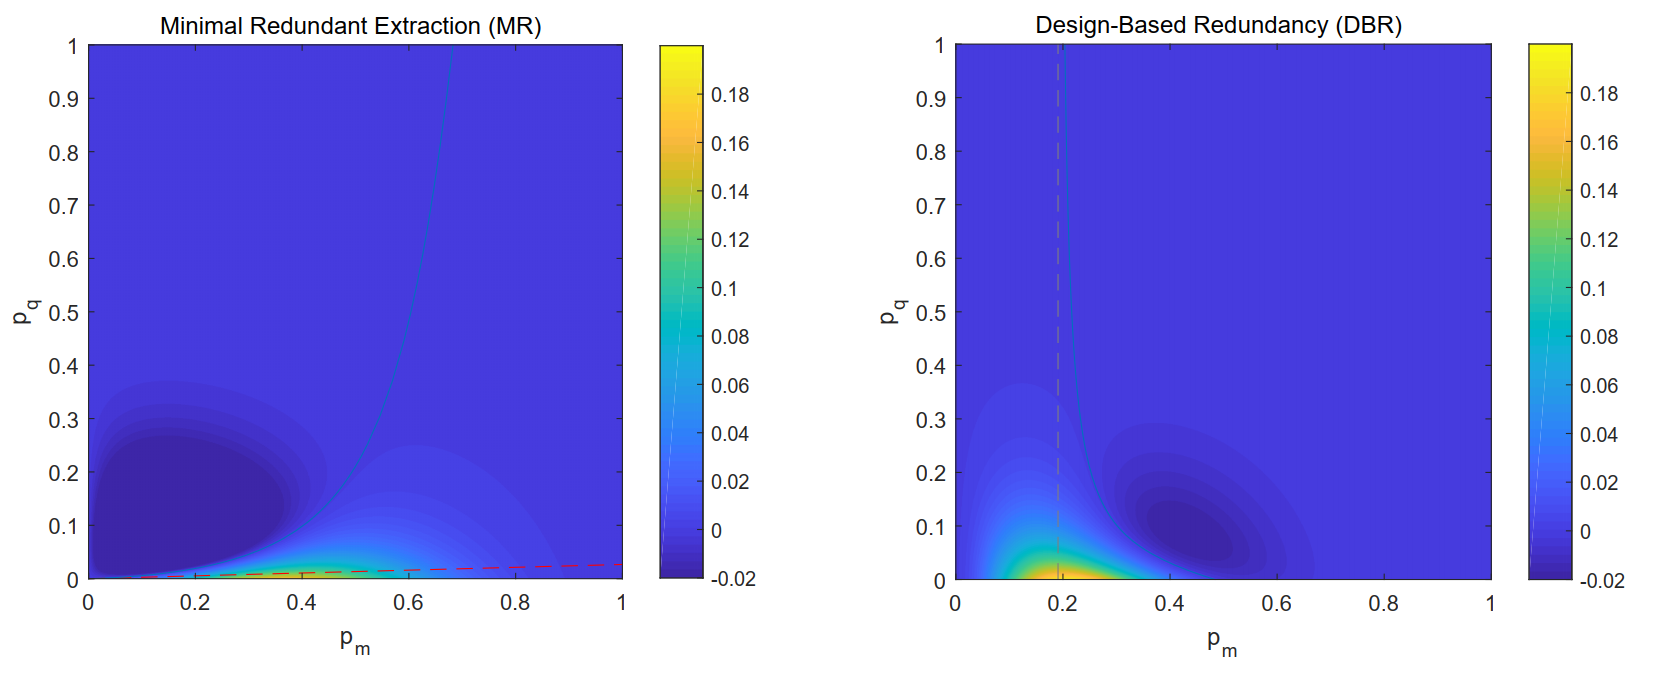
\includegraphics[width=\linewidth]{5_qubit_crop.PNG}
	\caption{$F_{QEC} - F_{MR}$ and $F_{QEC} - F_{DBR}$ for the [[5,1,3]] Perfect code. This is a zoomed-out version of the plot in the main text showing the results for all possible error rates.}
	\label{fig:5qubitperfectcodefullrange}
\end{figure}

\begin{figure}
	\centering
	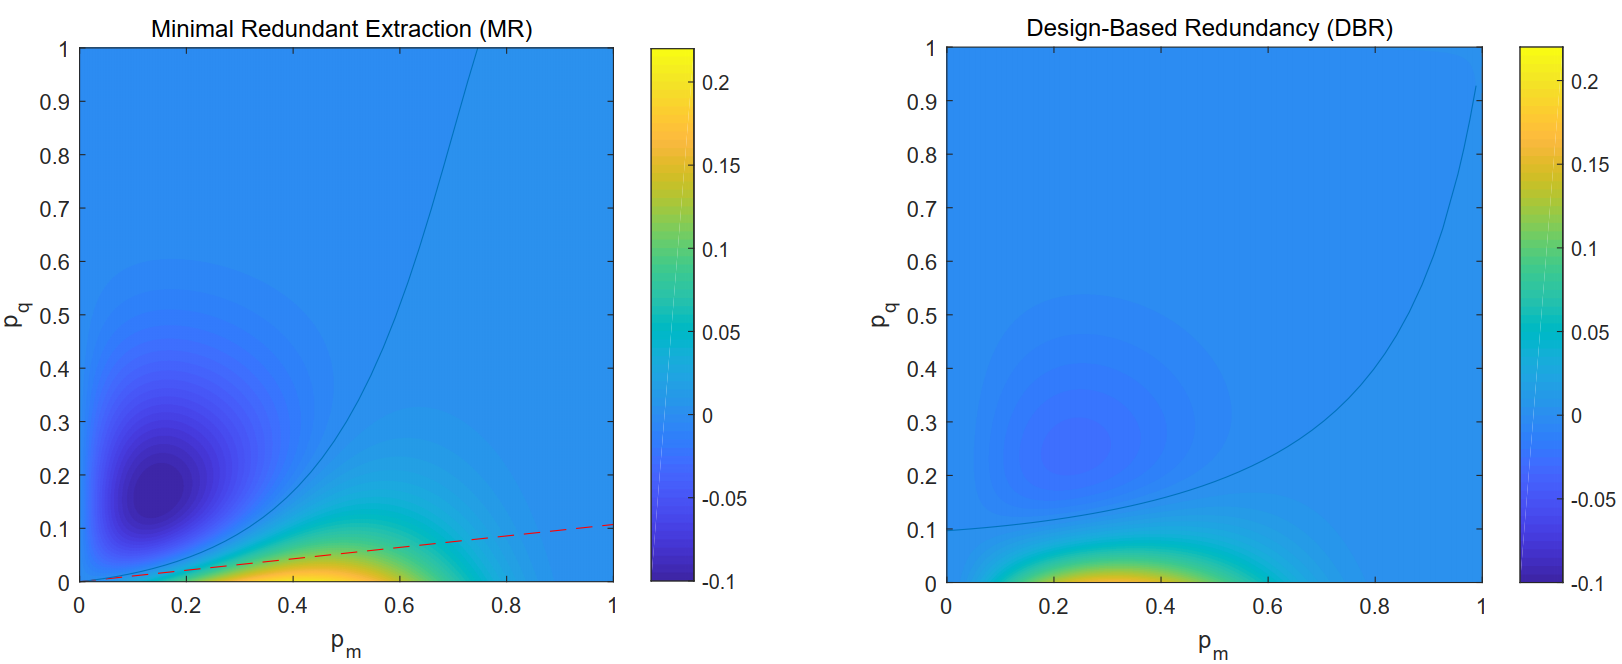
\includegraphics[width=\linewidth]{steane_crop.PNG}
	\caption{$F_{QEC} - F_{MR}$ and $F_{QEC} - F_{DBR}$ for the [[7,1,3]] Steane code. This is a zoomed-out version of the plot in the main text showing the results for all possible error rates.}
	\label{fig:steanecodefullrange}
\end{figure}

We also provided truncated analytic forms for the failure rates as a function of $p_q, p_m$, here we include the full expressions.

For 5-Qubit Perfect Code:

$F_{QEC} = 12p_{m}^{2} - 8p_{m}^{3} - 54p_{m}^{4} + 72p_{m}^{5} + 84p_{m}^{6} - 216p_{m}^{7} + 63p_{m}^{8} + 184p_{m}^{9} - 216p_{m}^{10} + 96p_{m}^{11} - 16p_{m}^{12} + 105p_{q}^{2} - 910p_{q}^{3} + 4095p_{q}^{4} - 12012p_{q}^{5} + 25025p_{q}^{6} - 38610p_{q}^{7} + 45045p_{q}^{8} - 40040p_{q}^{9} + 27027p_{q}^{10} - 13650p_{q}^{11} + 5005p_{q}^{12} - 1260p_{q}^{13} + 195p_{q}^{14} - 14p_{q}^{15} - 1260p_{m}^{2}p_{q}^{2} + 10920p_{m}^{2}p_{q}^{3} + 840p_{m}^{3}p_{q}^{2} - 49140p_{m}^{2}p_{q}^{4} - 7280p_{m}^{3}p_{q}^{3} + 5670p_{m}^{4}p_{q}^{2} + 144144p_{m}^{2}p_{q}^{5} + 32760p_{m}^{3}p_{q}^{4} - 49140p_{m}^{4}p_{q}^{3} - 7560p_{m}^{5}p_{q}^{2} - 300300p_{m}^{2}p_{q}^{6} - 96096p_{m}^{3}p_{q}^{5} + 221130p_{m}^{4}p_{q}^{4} + 65520p_{m}^{5}p_{q}^{3} - 8820p_{m}^{6}p_{q}^{2} + 463320p_{m}^{2}p_{q}^{7} + 200200p_{m}^{3}p_{q}^{6} - 648648p_{m}^{4}p_{q}^{5} - 294840p_{m}^{5}p_{q}^{4} + 76440p_{m}^{6}p_{q}^{3} + 22680p_{m}^{7}p_{q}^{2} - 540540p_{m}^{2}p_{q}^{8} - 308880p_{m}^{3}p_{q}^{7} + 1351350p_{m}^{4}p_{q}^{6} + 864864p_{m}^{5}p_{q}^{5} - 343980p_{m}^{6}p_{q}^{4} - 196560p_{m}^{7}p_{q}^{3} - 6615p_{m}^{8}p_{q}^{2} + 480480p_{m}^{2}p_{q}^{9} + 360360p_{m}^{3}p_{q}^{8} - 2084940p_{m}^{4}p_{q}^{7} - 1801800p_{m}^{5}p_{q}^{6} + 1009008p_{m}^{6}p_{q}^{5} + 884520p_{m}^{7}p_{q}^{4} + 57330p_{m}^{8}p_{q}^{3} - 19320p_{m}^{9}p_{q}^{2} - 324324p_{m}^{2}p_{q}^{10} - 320320p_{m}^{3}p_{q}^{9} + 2432430p_{m}^{4}p_{q}^{8} + 2779920p_{m}^{5}p_{q}^{7} - 2102100p_{m}^{6}p_{q}^{6} - 2594592p_{m}^{7}p_{q}^{5} - 257985p_{m}^{8}p_{q}^{4} + 167440p_{m}^{9}p_{q}^{3} + 22680p_{m}^{10}p_{q}^{2} + 163800p_{m}^{2}p_{q}^{11} + 216216p_{m}^{3}p_{q}^{10} - 2162160p_{m}^{4}p_{q}^{9} - 3243240p_{m}^{5}p_{q}^{8} + 3243240p_{m}^{6}p_{q}^{7} + 5405400p_{m}^{7}p_{q}^{6} + 756756p_{m}^{8}p_{q}^{5} - 753480p_{m}^{9}p_{q}^{4} - 196560p_{m}^{10}p_{q}^{3} - 10080p_{m}^{11}p_{q}^{2} - 60060p_{m}^{2}p_{q}^{12} - 109200p_{m}^{3}p_{q}^{11} + 1459458p_{m}^{4}p_{q}^{10} + 2882880p_{m}^{5}p_{q}^{9} - 3783780p_{m}^{6}p_{q}^{8} - 8339760p_{m}^{7}p_{q}^{7} - 1576575p_{m}^{8}p_{q}^{6} + 2210208p_{m}^{9}p_{q}^{5} + 884520p_{m}^{10}p_{q}^{4} + 87360p_{m}^{11}p_{q}^{3} + 1680p_{m}^{12}p_{q}^{2} + 15120p_{m}^{2}p_{q}^{13} + 40040p_{m}^{3}p_{q}^{12} - 737100p_{m}^{4}p_{q}^{11} - 1945944p_{m}^{5}p_{q}^{10} + 3363360p_{m}^{6}p_{q}^{9} + 9729720p_{m}^{7}p_{q}^{8} + 2432430p_{m}^{8}p_{q}^{7} - 4604600p_{m}^{9}p_{q}^{6} - 2594592p_{m}^{10}p_{q}^{5} - 393120p_{m}^{11}p_{q}^{4} - 14560p_{m}^{12}p_{q}^{3} - 2340p_{m}^{2}p_{q}^{14} - 10080p_{m}^{3}p_{q}^{13} + 270270p_{m}^{4}p_{q}^{12} + 982800p_{m}^{5}p_{q}^{11} - 2270268p_{m}^{6}p_{q}^{10} - 8648640p_{m}^{7}p_{q}^{9} - 2837835p_{m}^{8}p_{q}^{8} + 7104240p_{m}^{9}p_{q}^{7} + 5405400p_{m}^{10}p_{q}^{6} + 1153152p_{m}^{11}p_{q}^{5} + 65520p_{m}^{12}p_{q}^{4} + 168p_{m}^{2}p_{q}^{15} + 1560p_{m}^{3}p_{q}^{14} - 68040p_{m}^{4}p_{q}^{13} - 360360p_{m}^{5}p_{q}^{12} + 1146600p_{m}^{6}p_{q}^{11} + 5837832p_{m}^{7}p_{q}^{10} + 2522520p_{m}^{8}p_{q}^{9} - 8288280p_{m}^{9}p_{q}^{8} - 8339760p_{m}^{10}p_{q}^{7} - 2402400p_{m}^{11}p_{q}^{6} - 192192p_{m}^{12}p_{q}^{5} - 112p_{m}^{3}p_{q}^{15} + 10530p_{m}^{4}p_{q}^{14} + 90720p_{m}^{5}p_{q}^{13} - 420420p_{m}^{6}p_{q}^{12} - 2948400p_{m}^{7}p_{q}^{11} - 1702701p_{m}^{8}p_{q}^{10} + 7367360p_{m}^{9}p_{q}^{9} + 9729720p_{m}^{10}p_{q}^{8} + 3706560p_{m}^{11}p_{q}^{7} + 400400p_{m}^{12}p_{q}^{6} - 756p_{m}^{4}p_{q}^{15} - 14040p_{m}^{5}p_{q}^{14} + 105840p_{m}^{6}p_{q}^{13} + 1081080p_{m}^{7}p_{q}^{12} + 859950p_{m}^{8}p_{q}^{11} - 4972968p_{m}^{9}p_{q}^{10} - 8648640p_{m}^{10}p_{q}^{9} - 4324320p_{m}^{11}p_{q}^{8} - 617760p_{m}^{12}p_{q}^{7} + 1008p_{m}^{5}p_{q}^{15} - 16380p_{m}^{6}p_{q}^{14} - 272160p_{m}^{7}p_{q}^{13} - 315315p_{m}^{8}p_{q}^{12} + 2511600p_{m}^{9}p_{q}^{11} + 5837832p_{m}^{10}p_{q}^{10} + 3843840p_{m}^{11}p_{q}^{9} + 720720p_{m}^{12}p_{q}^{8} + 1176p_{m}^{6}p_{q}^{15} + 42120p_{m}^{7}p_{q}^{14} + 79380p_{m}^{8}p_{q}^{13} - 920920p_{m}^{9}p_{q}^{12} - 2948400p_{m}^{10}p_{q}^{11} - 2594592p_{m}^{11}p_{q}^{10} - 640640p_{m}^{12}p_{q}^{9} - 3024p_{m}^{7}p_{q}^{15} - 12285p_{m}^{8}p_{q}^{14} + 231840p_{m}^{9}p_{q}^{13} + 1081080p_{m}^{10}p_{q}^{12} + 1310400p_{m}^{11}p_{q}^{11} + 432432p_{m}^{12}p_{q}^{10} + 882p_{m}^{8}p_{q}^{15} - 35880p_{m}^{9}p_{q}^{14} - 272160p_{m}^{10}p_{q}^{13} - 480480p_{m}^{11}p_{q}^{12} - 218400p_{m}^{12}p_{q}^{11} + 2576p_{m}^{9}p_{q}^{15} + 42120p_{m}^{10}p_{q}^{14} + 120960p_{m}^{11}p_{q}^{13} + 80080p_{m}^{12}p_{q}^{12} - 3024p_{m}^{10}p_{q}^{15} - 18720p_{m}^{11}p_{q}^{14} - 20160p_{m}^{12}p_{q}^{13} + 1344p_{m}^{11}p_{q}^{15} + 3120p_{m}^{12}p_{q}^{14} - 224p_{m}^{12}p_{q}^{15}$

$F_{DBR} = 20475p_{m}^{4}p_{q} - 225225p_{m}^{5}p_{q} + 1126125p_{m}^{6}p_{q} - 3378375p_{m}^{7}p_{q} + 6756750p_{m}^{8}p_{q} - 9459450p_{m}^{9}p_{q} + 9459450p_{m}^{10}p_{q} - 6756750p_{m}^{11}p_{q} + 3378375p_{m}^{12}p_{q} - 1126125p_{m}^{13}p_{q} + 225225p_{m}^{14}p_{q} - 20475p_{m}^{15}p_{q} + 3003p_{m}^{5} - 25025p_{m}^{6} + 96525p_{m}^{7} - 225225p_{m}^{8} + 350350p_{m}^{9} - 378378p_{m}^{10} + 286650p_{m}^{11} - 150150p_{m}^{12} + 51975p_{m}^{13} - 10725p_{m}^{14} + 1001p_{m}^{15} + 105p_{q}^{2} - 910p_{q}^{3} + 4095p_{q}^{4} - 12012p_{q}^{5} + 25025p_{q}^{6} - 38610p_{q}^{7} + 45045p_{q}^{8} - 40040p_{q}^{9} + 27027p_{q}^{10} - 13650p_{q}^{11} + 5005p_{q}^{12} - 1260p_{q}^{13} + 195p_{q}^{14} - 14p_{q}^{15} - 286650p_{m}^{4}p_{q}^{2} + 1863225p_{m}^{4}p_{q}^{3} + 2837835p_{m}^{5}p_{q}^{2} - 7452900p_{m}^{4}p_{q}^{4} - 17762745p_{m}^{5}p_{q}^{3} - 13138125p_{m}^{6}p_{q}^{2} + 20495475p_{m}^{4}p_{q}^{5} + 69684615p_{m}^{5}p_{q}^{4} + 79704625p_{m}^{6}p_{q}^{3} + 37162125p_{m}^{7}p_{q}^{2} - 40990950p_{m}^{4}p_{q}^{6} - 189378189p_{m}^{5}p_{q}^{5} - 307432125p_{m}^{6}p_{q}^{4} - 219594375p_{m}^{7}p_{q}^{3} - 70945875p_{m}^{8}p_{q}^{2} + 61486425p_{m}^{4}p_{q}^{7} + 375750375p_{m}^{5}p_{q}^{6} + 826650825p_{m}^{6}p_{q}^{5} + 834458625p_{m}^{7}p_{q}^{4} + 409909500p_{m}^{8}p_{q}^{3} + 95645550p_{m}^{9}p_{q}^{2} - 70270200p_{m}^{4}p_{q}^{8} - 560404845p_{m}^{5}p_{q}^{7} - 1628251625p_{m}^{6}p_{q}^{6} - 2222295075p_{m}^{7}p_{q}^{5} - 1537160625p_{m}^{8}p_{q}^{4} - 541991450p_{m}^{9}p_{q}^{3} - 92702610p_{m}^{10}p_{q}^{2} + 61486425p_{m}^{4}p_{q}^{9} + 637702065p_{m}^{5}p_{q}^{8} + 2415538125p_{m}^{6}p_{q}^{7} + 4347968625p_{m}^{7}p_{q}^{6} + 4058104050p_{m}^{8}p_{q}^{5} + 2008556550p_{m}^{9}p_{q}^{4} + 516485970p_{m}^{10}p_{q}^{3} + 64496250p_{m}^{11}p_{q}^{2} - 40990950p_{m}^{4}p_{q}^{10} - 556110555p_{m}^{5}p_{q}^{9} - 2737609875p_{m}^{6}p_{q}^{8} - 6418429875p_{m}^{7}p_{q}^{7} - 7890757875p_{m}^{8}p_{q}^{6} - 5260505250p_{m}^{9}p_{q}^{5} - 1893781890p_{m}^{10}p_{q}^{4} - 354012750p_{m}^{11}p_{q}^{3} - 31531500p_{m}^{12}p_{q}^{2} + 20495475p_{m}^{4}p_{q}^{11} + 369738369p_{m}^{5}p_{q}^{10} + 2379752375p_{m}^{6}p_{q}^{9} + 7246614375p_{m}^{7}p_{q}^{8} + 11594583000p_{m}^{8}p_{q}^{7} + 10170310150p_{m}^{9}p_{q}^{6} + 4923832914p_{m}^{10}p_{q}^{5} + 1285625250p_{m}^{11}p_{q}^{4} + 170795625p_{m}^{12}p_{q}^{3} + 10308375p_{m}^{13}p_{q}^{2} - 7452900p_{m}^{4}p_{q}^{12} - 184459275p_{m}^{5}p_{q}^{11} - 1578151575p_{m}^{6}p_{q}^{10} - 6280399125p_{m}^{7}p_{q}^{9} - 13043905875p_{m}^{8}p_{q}^{8} - 14879714850p_{m}^{9}p_{q}^{7} - 9468909450p_{m}^{10}p_{q}^{6} - 3320266950p_{m}^{11}p_{q}^{5} - 614864250p_{m}^{12}p_{q}^{4} - 55180125p_{m}^{13}p_{q}^{3} - 2027025p_{m}^{14}p_{q}^{2} + 1863225p_{m}^{4}p_{q}^{13} + 66951885p_{m}^{5}p_{q}^{12} + 785659875p_{m}^{6}p_{q}^{11} + 4154725575p_{m}^{7}p_{q}^{10} + 11272511250p_{m}^{8}p_{q}^{9} + 16683316650p_{m}^{9}p_{q}^{8} + 13797553770p_{m}^{10}p_{q}^{7} + 6353597250p_{m}^{11}p_{q}^{6} + 1578151575p_{m}^{12}p_{q}^{5} + 197071875p_{m}^{13}p_{q}^{4} + 10735725p_{m}^{14}p_{q}^{3} + 181545p_{m}^{15}p_{q}^{2} - 286650p_{m}^{4}p_{q}^{14} - 16711695p_{m}^{5}p_{q}^{13} - 284659375p_{m}^{6}p_{q}^{12} - 2064187125p_{m}^{7}p_{q}^{11} - 7439857425p_{m}^{8}p_{q}^{10} - 14378714350p_{m}^{9}p_{q}^{9} - 15420795390p_{m}^{10}p_{q}^{8} - 9222963750p_{m}^{11}p_{q}^{7} - 3006003000p_{m}^{12}p_{q}^{6} - 502927425p_{m}^{13}p_{q}^{5} - 38063025p_{m}^{14}p_{q}^{4} - 952315p_{m}^{15}p_{q}^{3} + 20475p_{m}^{4}p_{q}^{15} + 2567565p_{m}^{5}p_{q}^{14} + 70945875p_{m}^{6}p_{q}^{13} + 746620875p_{m}^{7}p_{q}^{12} + 3689185500p_{m}^{8}p_{q}^{11} + 9468909450p_{m}^{9}p_{q}^{10} + 13256473230p_{m}^{10}p_{q}^{9} + 10277016750p_{m}^{11}p_{q}^{8} + 4347968625p_{m}^{12}p_{q}^{7} + 953827875p_{m}^{13}p_{q}^{6} + 96621525p_{m}^{14}p_{q}^{5} + 3353805p_{m}^{15}p_{q}^{4} - 183183p_{m}^{5}p_{q}^{15} - 10885875p_{m}^{6}p_{q}^{14} - 185810625p_{m}^{7}p_{q}^{13} - 1332205875p_{m}^{8}p_{q}^{12} - 4686631950p_{m}^{9}p_{q}^{11} - 8711396694p_{m}^{10}p_{q}^{10} - 8813054250p_{m}^{11}p_{q}^{9} - 4831076250p_{m}^{12}p_{q}^{8} - 1374998625p_{m}^{13}p_{q}^{7} - 182507325p_{m}^{14}p_{q}^{6} - 8471463p_{m}^{15}p_{q}^{5} + 775775p_{m}^{6}p_{q}^{15} + 28474875p_{m}^{7}p_{q}^{14} + 331080750p_{m}^{8}p_{q}^{13} + 1689738050p_{m}^{9}p_{q}^{12} + 4304049750p_{m}^{10}p_{q}^{11} + 5779723950p_{m}^{11}p_{q}^{10} + 4133254125p_{m}^{12}p_{q}^{9} + 1523647125p_{m}^{13}p_{q}^{8} + 262258425p_{m}^{14}p_{q}^{7} + 15940925p_{m}^{15}p_{q}^{6} - 2027025p_{m}^{7}p_{q}^{15} - 50675625p_{m}^{8}p_{q}^{14} - 419368950p_{m}^{9}p_{q}^{13} - 1549457910p_{m}^{10}p_{q}^{12} - 2850734250p_{m}^{11}p_{q}^{11} - 2705402700p_{m}^{12}p_{q}^{10} - 1300674375p_{m}^{13}p_{q}^{9} - 289864575p_{m}^{14}p_{q}^{8} - 22837815p_{m}^{15}p_{q}^{7} + 3603600p_{m}^{8}p_{q}^{15} + 64114050p_{m}^{9}p_{q}^{14} + 384053670p_{m}^{10}p_{q}^{13} + 1024773750p_{m}^{11}p_{q}^{12} + 1332205875p_{m}^{12}p_{q}^{11} + 849773925p_{m}^{13}p_{q}^{10} + 246921675p_{m}^{14}p_{q}^{9} + 25180155p_{m}^{15}p_{q}^{8} - 4554550p_{m}^{9}p_{q}^{15} - 58648590p_{m}^{10}p_{q}^{14} - 253685250p_{m}^{11}p_{q}^{13} - 478227750p_{m}^{12}p_{q}^{12} - 417792375p_{m}^{13}p_{q}^{11} - 161035875p_{m}^{14}p_{q}^{10} - 21406385p_{m}^{15}p_{q}^{9} + 4162158p_{m}^{10}p_{q}^{15} + 38697750p_{m}^{11}p_{q}^{14} + 118243125p_{m}^{12}p_{q}^{13} + 149774625p_{m}^{13}p_{q}^{12} + 79053975p_{m}^{14}p_{q}^{11} + 13936923p_{m}^{15}p_{q}^{10} - 2743650p_{m}^{11}p_{q}^{15} - 18018000p_{m}^{12}p_{q}^{14} - 36988875p_{m}^{13}p_{q}^{13} - 28303275p_{m}^{14}p_{q}^{12} - 6831825p_{m}^{15}p_{q}^{11} + 1276275p_{m}^{12}p_{q}^{15} + 5630625p_{m}^{13}p_{q}^{14} + 6981975p_{m}^{14}p_{q}^{13} + 2442895p_{m}^{15}p_{q}^{12} - 398475p_{m}^{13}p_{q}^{15} - 1061775p_{m}^{14}p_{q}^{14} - 601965p_{m}^{15}p_{q}^{13} + 75075p_{m}^{14}p_{q}^{15} + 91455p_{m}^{15}p_{q}^{14} - 6461p_{m}^{15}p_{q}^{15}$

$F_{MR} = 75p_{m}p_{q} - 1050p_{m}p_{q}^{2} - 300p_{m}^{2}p_{q} + 6825p_{m}p_{q}^{3} + 450p_{m}^{3}p_{q} - 27300p_{m}p_{q}^{4} - 300p_{m}^{4}p_{q} + 75075p_{m}p_{q}^{5} + 75p_{m}^{5}p_{q} - 150150p_{m}p_{q}^{6} + 225225p_{m}p_{q}^{7} - 257400p_{m}p_{q}^{8} + 225225p_{m}p_{q}^{9} - 150150p_{m}p_{q}^{10} + 75075p_{m}p_{q}^{11} - 27300p_{m}p_{q}^{12} + 6825p_{m}p_{q}^{13} - 1050p_{m}p_{q}^{14} + 75p_{m}p_{q}^{15} + 10p_{m}^{2} - 20p_{m}^{3} + 15p_{m}^{4} - 4p_{m}^{5} + 105p_{q}^{2} - 910p_{q}^{3} + 4095p_{q}^{4} - 12012p_{q}^{5} + 25025p_{q}^{6} - 38610p_{q}^{7} + 45045p_{q}^{8} - 40040p_{q}^{9} + 27027p_{q}^{10} - 13650p_{q}^{11} + 5005p_{q}^{12} - 1260p_{q}^{13} + 195p_{q}^{14} - 14p_{q}^{15} + 3150p_{m}^{2}p_{q}^{2} - 18200p_{m}^{2}p_{q}^{3} - 4200p_{m}^{3}p_{q}^{2} + 68250p_{m}^{2}p_{q}^{4} + 22750p_{m}^{3}p_{q}^{3} + 2625p_{m}^{4}p_{q}^{2} - 180180p_{m}^{2}p_{q}^{5} - 81900p_{m}^{3}p_{q}^{4} - 13650p_{m}^{4}p_{q}^{3} - 630p_{m}^{5}p_{q}^{2} + 350350p_{m}^{2}p_{q}^{6} + 210210p_{m}^{3}p_{q}^{5} + 47775p_{m}^{4}p_{q}^{4} + 3185p_{m}^{5}p_{q}^{3} - 514800p_{m}^{2}p_{q}^{7} - 400400p_{m}^{3}p_{q}^{6} - 120120p_{m}^{4}p_{q}^{5} - 10920p_{m}^{5}p_{q}^{4} + 579150p_{m}^{2}p_{q}^{8} + 579150p_{m}^{3}p_{q}^{7} + 225225p_{m}^{4}p_{q}^{6} + 27027p_{m}^{5}p_{q}^{5} - 500500p_{m}^{2}p_{q}^{9} - 643500p_{m}^{3}p_{q}^{8} - 321750p_{m}^{4}p_{q}^{7} - 50050p_{m}^{5}p_{q}^{6} + 330330p_{m}^{2}p_{q}^{10} + 550550p_{m}^{3}p_{q}^{9} + 353925p_{m}^{4}p_{q}^{8} + 70785p_{m}^{5}p_{q}^{7} - 163800p_{m}^{2}p_{q}^{11} - 360360p_{m}^{3}p_{q}^{10} - 300300p_{m}^{4}p_{q}^{9} - 77220p_{m}^{5}p_{q}^{8} + 59150p_{m}^{2}p_{q}^{12} + 177450p_{m}^{3}p_{q}^{11} + 195195p_{m}^{4}p_{q}^{10} + 65065p_{m}^{5}p_{q}^{9} - 14700p_{m}^{2}p_{q}^{13} - 63700p_{m}^{3}p_{q}^{12} - 95550p_{m}^{4}p_{q}^{11} - 42042p_{m}^{5}p_{q}^{10} + 2250p_{m}^{2}p_{q}^{14} + 15750p_{m}^{3}p_{q}^{13} + 34125p_{m}^{4}p_{q}^{12} + 20475p_{m}^{5}p_{q}^{11} - 160p_{m}^{2}p_{q}^{15} - 2400p_{m}^{3}p_{q}^{14} - 8400p_{m}^{4}p_{q}^{13} - 7280p_{m}^{5}p_{q}^{12} + 170p_{m}^{3}p_{q}^{15} + 1275p_{m}^{4}p_{q}^{14} + 1785p_{m}^{5}p_{q}^{13} - 90p_{m}^{4}p_{q}^{15} - 270p_{m}^{5}p_{q}^{14} + 19p_{m}^{5}p_{q}^{15}$

For Steane Code:

$F_{QEC} = 9p_{m}^{2} - 6p_{m}^{3} - 27p_{m}^{4} + 36p_{m}^{5} + 15p_{m}^{6} - 54p_{m}^{7} + 36p_{m}^{8}$

$F_{DBR} = 147p_{m}^{2}p_{q} - 735p_{m}^{3}p_{q} + 1470p_{m}^{4}p_{q} - 1470p_{m}^{5}p_{q} + 735p_{m}^{6}p_{q} - 147p_{m}^{7}p_{q} + 35p_{m}^{3} - 105p_{m}^{4} + 126p_{m}^{5} - 70p_{m}^{6} + 15p_{m}^{7} + 21p_{q}^{2} - 70p_{q}^{3} + 105p_{q}^{4} - 84p_{q}^{5} + 35p_{q}^{6} - 6p_{q}^{7} - 882p_{m}^{2}p_{q}^{2} + 2205p_{m}^{2}p_{q}^{3} + 3675p_{m}^{3}p_{q}^{2} - 2940p_{m}^{2}p_{q}^{4} - 8575p_{m}^{3}p_{q}^{3} - 6615p_{m}^{4}p_{q}^{2} + 2205p_{m}^{2}p_{q}^{5} + 11025p_{m}^{3}p_{q}^{4} + 14700p_{m}^{4}p_{q}^{3} + 6174p_{m}^{5}p_{q}^{2} - 882p_{m}^{2}p_{q}^{6} - 8085p_{m}^{3}p_{q}^{5} - 18375p_{m}^{4}p_{q}^{4} - 13230p_{m}^{5}p_{q}^{3} - 2940p_{m}^{6}p_{q}^{2} + 147p_{m}^{2}p_{q}^{7}  3185p_{m}^{3}p_{q}^{6} + 13230p_{m}^{4}p_{q}^{5}  16170p_{m}^{5}p_{q}^{4} + 6125p_{m}^{6}p_{q}^{3}  567p_{m}^{7}p_{q}^{2} - 525p_{m}^{3}p_{q}^{7}  5145p_{m}^{4}p_{q}^{6}  11466p_{m}^{5}p_{q}^{5}$

$F_{MR} = 28p_{m}p_{q} - 168p_{m}p_{q}^{2} - 84p_{m}^{2}p_{q} + 420p_{m}p_{q}^{3} + 84p_{m}^{3}p_{q} - 560p_{m}p_{q}^{4} - 28p_{m}^{4}p_{q} + 420p_{m}p_{q}^{5} - 168p_{m}p_{q}^{6} + 28p_{m}p_{q}^{7} + 6p_{m}^{2} - 8p_{m}^{3} + 3p_{m}^{4} + 21p_{q}^{2} - 70p_{q}^{3} + 105p_{q}^{4} - 84p_{q}^{5} + 35p_{q}^{6} - 6p_{q}^{7} + 378p_{m}^{2}p_{q}^{2} - 840p_{m}^{2}p_{q}^{3} - 336p_{m}^{3}p_{q}^{2} + 1050p_{m}^{2}p_{q}^{4} + 700p_{m}^{3}p_{q}^{3} + 105p_{m}^{4}p_{q}^{2} - 756p_{m}^{2}p_{q}^{5} - 840p_{m}^{3}p_{q}^{4} - 210p_{m}^{4}p_{q}^{3} + 294p_{m}^{2}p_{q}^{6} + 588p_{m}^{3}p_{q}^{5} + 245p_{m}^{4}p_{q}^{4} - 48p_{m}^{2}p_{q}^{7}  224p_{m}^{3}p_{q}^{6}$




For Bitflip Code:

$F_{QEC} = 6p_{m}^{2} - 4p_{m}^{3} - 9p_{m}^{4} + 12p_{m}^{5} - 4p_{m}^{6} + 3p_{q}^{2} - 2p_{q}^{3} - 18p_{m}^{2}p_{q}^{2} + 12p_{m}^{2}p_{q}^{3} + 12p_{m}^{3}p_{q}^{2} - 8p_{m}^{3}p_{q}^{3} + 27p_{m}^{4}p_{q}^{2} - 18p_{m}^{4}p_{q}^{3} - 36p_{m}^{5}p_{q}^{2} + 24p_{m}^{5}p_{q}^{3} + 12p_{m}^{6}p_{q}^{2}$

$F_{DBR} = 9p_{m}p_{q} - 18p_{m}p_{q}^{2} - 18p_{m}^{2}p_{q} + 9p_{m}p_{q}^{3} + 9p_{m}^{3}p_{q} + 3p_{m}^{2} - 2p_{m}^{3} + 3p_{q}^{2} - 2p_{q}^{3} + 27p_{m}^{2}p_{q}^{2} - 12p_{m}^{2}p_{q}^{3} - 12p_{m}^{3}p_{q}^{2} + 5p_{m}^{3}p_{q}^{3}$

\end{document}
